The idea is to build during preprocessing a graph inspired in the Itemset Lattice that describes the influence of
different categorical relations on a given numerical attribute's distribution. We call such graph a \graphname.
Comparing to a Itemset Lattice, in a \graphname we have a set categorical relations (that are joined with root
attribute) instead of items. In addition, Each node in the graph has a associated histogram with the support
distribution over the root's numerical attribute.

To illustrate the idea, let's analyze a simple real-world example with the \emph{hasIncome} relation. If we have two
categorical relations, one strongly correlated to income, e.g. \emph{hasEducation}, and one uncorrelated (or very weakly
correlated), e.g. \emph{wasBornInMonth}.

Let's assume that for the relation \emph{wasBornInMonth(x,y)} we have the 12 months from the Gregorian Calendar as
constants and for \emph{hasEducation(x,y)} we can have 10 different categorical constants for \emph{y}: ``Preschool'',
``Kindergarten'', ``ElementarySchool'', ``MiddleSchool'', ``Highschool'', ``Professional School'', ``Associate's
degree'', ``Bachelor's degree'', ``Master's degree'' and ``Doctorate degree''. 

It's expected that the income distribution will be roughly the same for people born in any of the months, whereas
for different education levels, e.g. Elementary School and Doctoral Degree, their income distribution are expected to be
different between them and different from the overall income distribution.

In a further step, we try to join every possible pair of categorical relations and including the constants. For the
given, example with the relations \emph{hasEducation} and \emph{wasBornInMonth} we would then create the nodes:

  \emph{hasIncome(x,y)wasBornInMonth(x,``January''),hasEducation(x,``Preschool'')} \newline
  \emph{hasIncome(x,y)wasBornInMonth(x,``January''),hasEducation(x,``Kindergarten'')} \newline
  \dots \newline
  \emph{hasIncome(x,y)wasBornInMonth(x,``January''),hasEducation(x,``Doctorate Degree'')} \newline

  \emph{hasIncome(x,y)wasBornInMonth(x,``February''),hasEducation(x,``Preschool'')} \newline
  \emph{hasIncome(x,y)wasBornInMonth(x,``February''),hasEducation(x,``Kindergarten'')} \newline
  \dots \newline
  \emph{hasIncome(x,y)wasBornInMonth(x,``February''),hasEducation(x,``Doctorate Degree'')} \newline
 
  \dots \newline

  \emph{hasIncome(x,y)wasBornInMonth(x,``December''),hasEducation(x,``Preschool'')} \newline
  \emph{hasIncome(x,y)wasBornInMonth(x,``December''),hasEducation(x,``Kindergarten'')} \newline
  \dots \newline
  \emph{hasIncome(x,y)wasBornInMonth(x,``December''),hasEducation(x,``Doctorate Degree'')} \newline


Based on this idea, we basically check how different categorical relations affect a numerical distribution. Such
information, together with other measures like support, provides valuable cues on what categorical attributes and what
categorical constants might be the most interesting to be added to the hypothesis in the core ILP algorithm.

\ref{fig:lattice} shows how a \graphname looks like.

\begin{figure}[!h]
  \caption{Correlation Lattice example}
  \centering
  \begin{tikzpicture}
 [scale=1.8,auto=center,every node/.style={minimum, font=\tiny}]
  \node (n0) at (4,10) {$r$};
  \node (na) at (0,8)  {$r a$};
  \node (na1)%[fill=blue!20] 
  at (1,7.5)  {$r a_1$};
  \node (na2)%[fill=blue!20] 
  at (2,7.5) {$r a_2$};
  \node (nb) at (3,8)  {$r b$};
  \node (nb1)%[fill=red!20] 
  at (4,7.5)  {$r b_1$};
  \node (nb2)%[fill=red!20] 
  at (5,7.5)  {$r b_1$};
  \node (nc) at (6,8)  {$r c$};
  \node (nc1)%[fill=green!20] 
  at (7,7.5)  {$r c_1$};
  \node (nc2)%[fill=green!20] 
  at (8,7.5)  {$r c_1$};
  \node (nab) at (0,5)  {$r a b$};
  \node (na1b1)%[fill=magenta!20] 
  at (0.5,4.5)  {$r a_1 b_1$};
  \node (na1b2)%[fill=magenta!20] 
  at (1.0,4.5)  {$r a_1 b_2$};
  \node (na2b1)%[fill=magenta!20] 
  at (1.5,4.5)  {$r a_2 b_1$};
  \node (na2b2)%[fill=magenta!20] 
  at (2.0,4.5)  {$r a_2 b_2$};
  \node (nac) at (3,5)  {$r a c$};
  \node (na1c1)%[fill=cyan!20] 
  at (3.5,4.5)  {$r a_1 c_1$};
  \node (na1c2)%[fill=cyan!20] 
  at (4.0,4.5)  {$r a_1 c_2$};
  \node (na2c1)%[fill=cyan!20] 
  at (4.5,4.5)  {$r a_2 c_1$};
  \node (na2c2)%[fill=cyan!20] 
  at (5.0,4.5)  {$r a_2 c_2$};
  \node (nbc) at (6,5)  {$r b c$};
  \node (nb1c1)%[fill=yellow!50] 
  at (6.5,4.5)  {$r b_1 c_1$};
  \node (nb1c2)%[fill=yellow!50] 
  at (7.0,4.5)  {$r b_1 c_2$};
  \node (nb2c1)%[fill=yellow!50] 
  at (7.5,4.5)  {$r b_2 c_1$};
  \node (nb2c2)%[fill=yellow!50] 
  at (8.0,4.5)  {$r b_2 c_2$};
  \node (nabc) at (2,2)  {$r a b c$};
  \node (na1b1c1)%[fill=black!10] 
  at (2.5,1.5)  {$r a_1 b_1 c_1$};
  \node (na1b1c2)%[fill=black!10] 
  at (3.2,1.5)  {$r a_1 b_1 c_2$};
  \node (na1b2c1)%[fill=black!10] 
  at (3.9,1.5)  {$r a_1 b_2 c_1$};  
  \node (na1b2c2)%[fill=black!10] 
  at (4.6,1.5)  {$r a_1 b_2 c_2$};
  \node (na2b1c1)%[fill=black!10] 
  at (5.3,1.5)  {$r a_2 b_1 c_1$};
  \node (na2b1c2)%[fill=black!10] 
  at (6.0,1.5)  {$r a_2 b_1 c_2$};
  \node (na2b2c1)%[fill=black!10] 
  at (6.7,1.5)  {$r a_2 b_2 c_1$};
  \node (na2b2c2)%[fill=black!10] 
  at (7.4,1.5)  {$r a_2 b_2 c_2$};

  \foreach \from/\to in {na/na1,na/na2,nb/nb1,nb/nb2,nc/nc1,nc/nc2}
    \draw[dashed] (\from) -| (\to);

  \foreach \from/\to in {nab/na1b1,nab/na1b2,nab/na2b1,nab/na2b2}
    \draw[dashed] (\from) -| (\to);

  \foreach \from/\to in {nabc/na1b1c1,nabc/na1b1c2,nabc/na1b2c1,nabc/na1b2c2,nabc/na2b1c1,nabc/na2b1c2,nabc/na2b2c1,nabc/na2b2c2}
    \draw[dashed] (\from) -| (\to);

  \foreach \from/\to in {n0/na1,n0/na2,na1/na1b1,na1/na1b2,na2/na2b1,na2/na2b2,na1/na1c1,na1/na1c2,na2/na2c1,na2/na2c2}
    \draw[blue] (\from) -- (\to);
  \foreach \from/\to in {n0/nb1,n0/nb2,nb1/na1b1,nb1/na2b1,nb2/na1b2,nb2/na2b2,nb1/nb1c1,nb1/nb1c2,nb2/nb2c1,nb2/nb2c2}
    \draw[red] (\from) -- (\to);
  \foreach \from/\to in {n0/nc1,n0/nc2,nc1/na1c1,nc1/na2c1,nc2/na1c2,nc2/na2c2,nc1/nb1c1,nc1/nb2c1,nc2/nb1c2,nc2/nb2c2}
    \draw[green] (\from) -- (\to);
  \foreach \from/\to in {na1b1/na1b1c1,na1b2/na1b2c1,na2b1/na2b1c1,na2b2/na2b2c1,na1b1/na1b1c2,na1b2/na1b2c2,na2b1/na2b1c2,na2b2/na2b2c2}
    \draw[magenta] (\from) -- (\to);
  \foreach \from/\to in {na1c1/na1b1c1,na1c1/na1b2c1,na2c1/na2b1c1,na2c1/na2b2c1,na1c2/na1b1c2,na1c2/na1b2c2,na2c2/na2b1c2,na2c2/na2b2c2}
    \draw[cyan] (\from) -- (\to);
  \foreach \from/\to in {nb1c1/na1b1c1,nb2c1/na1b2c1,nb1c1/na2b1c1,nb2c1/na2b2c1,nb1c2/na1b1c2,nb2c2/na1b2c2,nb1c2/na2b1c2,nb2c2/na2b2c2}
    \draw[yellow] (\from) -- (\to);

  \foreach \from/\to in {n0/na,n0/nb,n0/nc}
    \draw[dashed] (\from) -- (\to);
  \foreach \from/\to in {na/nab,na/nac,nb/nab,nb/nbc,nc/nac,nc/nbc,nab/nabc,nac/nabc,nbc/nabc}
    \draw[dashed] (\from) -- (\to);  
\end{tikzpicture}

  \label{fig:lattice}
\end{figure}

\subsection{Pruning Opportunities}

In this section we discuss about safe pruning opportunities that can be explored whilst building the \graphname: support
and conditional independence. As these might not be sufficient to reduce lattice size to a feasible level, later, in
section(??), we will also discuss possible pruning techniques.

\subsubsection{Support}

As described in (\cite{LavracDz94}), in top-down ILP every refinement causes the support to decrease, therefore we know
that for every node in the \graphname, its support will be greater or equal than any of its children, so support is a
monotonically decreasing measure so we can safely prune a node that doesn't reach the minimum support threshold.

In this thesis, we define support as the absolute frequency of supporting facts.


\subsubsection{Independence Checks}

By simplicity, we assume that every possible pair of categorical relations are independent given their common parent and
we search for evidence to prove the contrary.

For 2 nodes to be joined, they must have a common parent, i.e. two nodes at level $l$ (with $l+1$ literals) are joinable
if they share $l$ literals. Therefore, it's straightforward to calculate the conditional probabilities of each of the
joining nodes given the common parent, and estimate the frequency distribution for the conditional independence case.

If we are joining hasEducation()...

Let's say we have the following join case:
 
\begin{figure}[!h]
  \caption{Node join example for independence test}
  \centering
  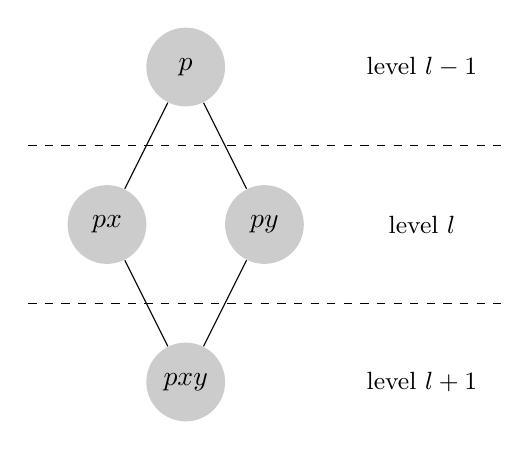
\begin{tikzpicture}
  [scale=1,auto=center,every node/.style={minimum size=1cm}]
    \node (p)  [circle,fill=black!20] at (4,10) {$p$};
    \node (n1) [circle,fill=black!20] at (3,8)  {$p x$};
    \node (n2) [circle,fill=black!20] at (5,8)  {$p y$};
    \node (n12)[circle,fill=black!20] at (4,6)  {$p x y$};


    \foreach \from/\to in {p/n1,p/n2,n1/n12,n2/n12}
      \draw (\from) -- (\to);

    \draw[dashed] (2,9) -- (8,9);
    \draw[dashed] (2,7) -- (8,7);

    \node (level0)[font=\small] at (7,10) {level $l-1$};
    \node (level1)[font=\small] at (7,8)  {level $l$};
    \node (level2)[font=\small] at (7,6)  {level $l+1$};
  \end{tikzpicture}
  \label{fig:joinIndepExample}
\end{figure}

For the example shown in ~\ref{fig:joinIndepExample}, we can calculate the conditional probability $p_i(x|p)$ and
$p_i(y|p)$ assuming conditional independence given common parent $p$ in order to estimate $\hat{h_i}(p x y)$:

\begin{equation}
\label{eq:condindep}
\begin{split}
 p_i(x|py) &= p_i(x|p) \\ 
 &= \cfrac{h_i(x)}{h_i(p)} \\ 
 p_i(y|px) &= p_i(y|p) \\ 
 &= \cfrac{h_i(y)}{h_i(p)} \\ \\ 
 \hat{h_i}(pxy) &= p_i(x|py)p_i(y|p)*h_i(p) \\ 
 &= p_i(x|p)h_i(y) \\ 
 \hat{h_i}(pxy) &= p_i(y|px)p_i(x|p)*h_i(p) \\ 
 &= p_i(y|p)h_i(x) 
\end{split}
\end{equation}

After that, we query the actual frequency distribution on the Knowledge Base and do an Pearson's chi-squared
independence test. As null hypothesis and alternative hypothesis we have:

\begin{itemize}
 \item $H_0$ = \emph{$x$ and $y$ are conditionally independent given their common parent $p$}
 \item $H_1$ = \emph{$x$ and $y$ are conditionally dependent given their common parent $p$} 
\end{itemize}

Number of degrees of freedom is the number of buckets minus one:

\begin{center}
 $df=k-1$
\end{center}

We calculate the $\chi^2$ value:

\begin{equation}
 \chi^2=\sum_{i=1}^{k} \cfrac{(h_i - \hat{h_i})^2}{\hat{h_i}}
\end{equation}

\cite{Jaroszewicz02pruningredundant}

Then it's possible to obtain the p-value and check whether there's enough confidence to reject the null hypothesis
$H_0$. 


In other words if we find out that $x$ and $y$ are conditionally independent given $p$, we could rewrite the equation
\ref{eq:condindep} as the following rules being equivalents, with similar accuracy distributions:

$x \leftarrow py \equiv x \leftarrow p$
$y \leftarrow px \equiv y \leftarrow p$

Therefore, we know that if we have $x$ fixed as head of clauses in the core ILP, and we currently have $x \leftarrrow
p$, joining the node $px$ with $py$ to obtain the rule $x \leftarrow py$ doesn't add any information. The same applies
for having $y$, and obtaining $y \leftarrow px$ from $y \leftarrow p$ by joining the same pair of nodes. This property
plays an important role in the integration of the correlation lattice into the core ILP as we will explain in more
details later in Section (???).

Nevertheless cannot be safely pruned from the lattice.  


In level 1 from \graphname, nodes can be directly pruned, on the other hand, for further levels, for a node to be
pruned by independence, all the possible joins resulting the node must be independent. In level 2, for example, in order
to prune the node $r a_1 b_1 c_1$, given that in level 1 the nodes $r a_1 b_1$, $r a_1 c_1$ and $r b_1 c_1$ were not
pruned. All the three possible join combinations should fail the independence test, i.e.:

\begin{equation}
\begin{split} 
  freq(r a_1 b_1 c_1) &\approx freq(r a_1)p (r b_1|r a_1) p(r c_1|r a_1) \\ 
  &\approx  freq(r b_1) p(r a_1|r b_1) p(r c_1|r b_1) \\ 
  &\approx  freq(r c_1) p(r a_1|r c_1) p(r b_1|r c_1)  
\end{split}
\end{equation}

This applies to nodes at any level $l$, with $p \leq l$ parents and $C_{2}^{p}$ possible join pairs.

If any of the join pairs has enough evidence of being dependent, then 2 edges are created connecting each of the joined
nodes to the result of their join

\subsection{Distribution Divergence Measures}

As seen in the previous sections, we are interested in rules whose base-rule has accuracy bellow threshold,
but for one or multiple specific intervals with accuracy above threshold. For this to happen, we need a rule with
non-uniform accuracy distribution, or in other words, divergent body and positive examples distributions.

Therefore,we are interested in adding categories that produces distributions different from the their
parent nodes. In other to measure such divergence between distributions, some of the state-of-the-art such as the
following ones can be used.

\begin{itemize}
 \item Kullback-Leibler \cite{Kullback51klDivergence}: 
    \begin{equation}
      D_{KL}(P||Q)=\sum_{\substack{i}}\ln\left(\cfrac{P(i)}{Q(i)}\right)*P(i)
    \end{equation}
 \item Chi-squared ($\chi^2$):
    \begin{equation}
      D_{\chi^2}(P||Q)=\sum_{\substack{i}}\cfrac{(P(i)-Q(i))^2}{P(i)}
    \end{equation}
 \item Jensen-Shannon \cite{17795}:
    \begin{equation}
      D_{JS}(P||Q)=\cfrac{1}{2}D_{KL}(P||M)+\cfrac{1}{2}D_{KL}(Q||M), 
    \end{equation}
\end{itemize}

Where $P$ and $Q$ are the distributions to be compared and $M=\cfrac{1}{2}(P+Q)$

As discussed in \cite{17795}, although Jensen-Shannon is computationally more expensive, it has the advantage of being a
symmetric and smoothed version of the Kullback-Leibler measure.


\subsection{Heuristics}

As seen before, the number of nodes in \graphname grow exponentially with the number of categorical relations
and its constants. For $n$ categorical relations, each with $m$ constants, the total number of nodes is $2^{nm}$.
Frequently, pruning by support and independence is not sufficient to make it feasible and it's necessary to apply
heuristics to prune more aggressively.

%%% Divergence

Pruning by divergence is clearly not safe. Let's suppose we have a root numerical property $r(x,y)$, and two categorical
relations $a(x,z)$ with constants $A_1$ and $A_2$ and $b(x,w)$ with constants $B_1$ and $B_2$. For simplicity, let's
assume y is divided in two buckets and root $r$ has an uniform distribution $[0.5 \, 0.5]$ from frequencies $[2 \, 2]$.
It's possible to have $r a_1$ and $r a_2$ as well as $r b_1$ and $r b_2$ with the same uniform distribution with
frequencies $[1 \, 1]$. Nevertheless when combined we can have the following:

$r a_1 b_1 : [1.0 \, 0.0] \\$
$r a_1 b_2 : [0.0 \, 1.0] \\$
$r a_2 b_1 : [0.0 \, 1.0] \\$
$r a_2 b_2 : [1.0 \, 0.0]$

As shown above, divergence is not a monotonically decreasing measure, thus it can only be used as heuristics.

% Draw example instead to explain better

Moreover, using a divergence measure alone might also be problematic. Nodes with low support are more likely to
present high divergence and then nodes with high support, supposing that they were drawn under the same distribution.
Therefore, it's important to use divergence combined with support as pruning heuristics.

Moreover, we are interested not only in rules with high confidence, but also rules with high support so more facts can
be derived.

% Talk about how to use such measure? (Threshold, Top-k, Cost-Benefit)

%%% Independence

As seen seen in Section (???), checking for conditional independence of categories is very insightful and
can detect equivalent rules like in Figure \ref{fig:joinIndepExample} where we know that $x \leftarrow py \equiv x
\leftarrow p$ and $y \leftarrow px \equiv y \leftarrow p$. Nevertheless, we cannot prune the node $pxy$ from the
lattice as we $x$ and $y$ might not be independent given $pz$, and for instance, a rule $x \leftarrow pyz$ might not be
equivalent to $x \leftarrow py$. 



